\documentclass[conference]{IEEEtran}
% Add the compsoc option for Computer Society conferences.
%
% If IEEEtran.cls has not been installed into the LaTeX system files,
% manually specify the path to it like:
% \documentclass[conference]{../sty/IEEEtran}





% Some very useful LaTeX packages include:
% (uncomment the ones you want to load)


% *** MISC UTILITY PACKAGES ***
%
%\usepackage{ifpdf}
% Heiko Oberdiek's ifpdf.sty is very useful if you need conditional
% compilation based on whether the output is pdf or dvi.
% usage:
% \ifpdf
%   % pdf code
% \else
%   % dvi code
% \fi
% The latest version of ifpdf.sty can be obtained from:
% http://www.ctan.org/tex-archive/macros/latex/contrib/oberdiek/
% Also, note that IEEEtran.cls V1.7 and later provides a builtin
% \ifCLASSINFOpdf conditional that works the same way.
% When switching from latex to pdflatex and vice-versa, the compiler may
% have to be run twice to clear warning/error messages.






% *** CITATION PACKAGES ***
%
%\usepackage{cite}
% cite.sty was written by Donald Arseneau
% V1.6 and later of IEEEtran pre-defines the format of the cite.sty package
% \cite{} output to follow that of IEEE. Loading the cite package will
% result in citation numbers being automatically sorted and properly
% "compressed/ranged". e.g., [1], [9], [2], [7], [5], [6] without using
% cite.sty will become [1], [2], [5]--[7], [9] using cite.sty. cite.sty's
% \cite will automatically add leading space, if needed. Use cite.sty's
% noadjust option (cite.sty V3.8 and later) if you want to turn this off.
% cite.sty is already installed on most LaTeX systems. Be sure and use
% version 4.0 (2003-05-27) and later if using hyperref.sty. cite.sty does
% not currently provide for hyperlinked citations.
% The latest version can be obtained at:
% http://www.ctan.org/tex-archive/macros/latex/contrib/cite/
% The documentation is contained in the cite.sty file itself.






% *** GRAPHICS RELATED PACKAGES ***
%
\ifCLASSINFOpdf
  \usepackage[pdftex]{graphicx}
  % declare the path(s) where your graphic files are
  % \graphicspath{{../pdf/}{../jpeg/}}
  % and their extensions so you won't have to specify these with
  % every instance of \includegraphics
  % \DeclareGraphicsExtensions{.pdf,.jpeg,.png}
\else
  % or other class option (dvipsone, dvipdf, if not using dvips). graphicx
  % will default to the driver specified in the system graphics.cfg if no
  % driver is specified.
  % \usepackage[dvips]{graphicx}
  % declare the path(s) where your graphic files are
  % \graphicspath{{../eps/}}
  % and their extensions so you won't have to specify these with
  % every instance of \includegraphics
  % \DeclareGraphicsExtensions{.eps}
\fi
% graphicx was written by David Carlisle and Sebastian Rahtz. It is
% required if you want graphics, photos, etc. graphicx.sty is already
% installed on most LaTeX systems. The latest version and documentation can
% be obtained at: 
% http://www.ctan.org/tex-archive/macros/latex/required/graphics/
% Another good source of documentation is "Using Imported Graphics in
% LaTeX2e" by Keith Reckdahl which can be found as epslatex.ps or
% epslatex.pdf at: http://www.ctan.org/tex-archive/info/
%
% latex, and pdflatex in dvi mode, support graphics in encapsulated
% postscript (.eps) format. pdflatex in pdf mode supports graphics
% in .pdf, .jpeg, .png and .mps (metapost) formats. Users should ensure
% that all non-photo figures use a vector format (.eps, .pdf, .mps) and
% not a bitmapped formats (.jpeg, .png). IEEE frowns on bitmapped formats
% which can result in "jaggedy"/blurry rendering of lines and letters as
% well as large increases in file sizes.
%
% You can find documentation about the pdfTeX application at:
% http://www.tug.org/applications/pdftex





% *** MATH PACKAGES ***
%
%\usepackage[cmex10]{amsmath}
% A popular package from the American Mathematical Society that provides
% many useful and powerful commands for dealing with mathematics. If using
% it, be sure to load this package with the cmex10 option to ensure that
% only type 1 fonts will utilized at all point sizes. Without this option,
% it is possible that some math symbols, particularly those within
% footnotes, will be rendered in bitmap form which will result in a
% document that can not be IEEE Xplore compliant!
%
% Also, note that the amsmath package sets \interdisplaylinepenalty to 10000
% thus preventing page breaks from occurring within multiline equations. Use:
%\interdisplaylinepenalty=2500
% after loading amsmath to restore such page breaks as IEEEtran.cls normally
% does. amsmath.sty is already installed on most LaTeX systems. The latest
% version and documentation can be obtained at:
% http://www.ctan.org/tex-archive/macros/latex/required/amslatex/math/





% *** SPECIALIZED LIST PACKAGES ***
%
\usepackage[longend,linesnumbered]{algorithm2e}
\usepackage{algorithmic}


\newcommand{\code}[1]{\lstset{basicstyle=\small\tt}\lstinline£#1£\lstset
{basicstyle=\footnotesize\tt}}

% algorithmic.sty was written by Peter Williams and Rogerio Brito.
% This package provides an algorithmic environment fo describing algorithms.
% You can use the algorithmic environment in-text or within a figure
% environment to provide for a floating algorithm. Do NOT use the algorithm
% floating environment provided by algorithm.sty (by the same authors) or
% algorithm2e.sty (by Christophe Fiorio) as IEEE does not use dedicated
% algorithm float types and packages that provide these will not provide
% correct IEEE style captions. The latest version and documentation of
% algorithmic.sty can be obtained at:
% http://www.ctan.org/tex-archive/macros/latex/contrib/algorithms/
% There is also a support site at:
% http://algorithms.berlios.de/index.html
% Also of interest may be the (relatively newer and more customizable)
% algorithmicx.sty package by Szasz Janos:
% http://www.ctan.org/tex-archive/macros/latex/contrib/algorithmicx/




% *** ALIGNMENT PACKAGES ***
%
%\usepackage{array}
% Frank Mittelbach's and David Carlisle's array.sty patches and improves
% the standard LaTeX2e array and tabular environments to provide better
% appearance and additional user controls. As the default LaTeX2e table
% generation code is lacking to the point of almost being broken with
% respect to the quality of the end results, all users are strongly
% advised to use an enhanced (at the very least that provided by array.sty)
% set of table tools. array.sty is already installed on most systems. The
% latest version and documentation can be obtained at:
% http://www.ctan.org/tex-archive/macros/latex/required/tools/


%\usepackage{mdwmath}
%\usepackage{mdwtab}
% Also highly recommended is Mark Wooding's extremely powerful MDW tools,
% especially mdwmath.sty and mdwtab.sty which are used to format equations
% and tables, respectively. The MDWtools set is already installed on most
% LaTeX systems. The lastest version and documentation is available at:
% http://www.ctan.org/tex-archive/macros/latex/contrib/mdwtools/


% IEEEtran contains the IEEEeqnarray family of commands that can be used to
% generate multiline equations as well as matrices, tables, etc., of high
% quality.


%\usepackage{eqparbox}
% Also of notable interest is Scott Pakin's eqparbox package for creating
% (automatically sized) equal width boxes - aka "natural width parboxes".
% Available at:
% http://www.ctan.org/tex-archive/macros/latex/contrib/eqparbox/





% *** SUBFIGURE PACKAGES ***
%\usepackage[tight,footnotesize]{subfigure}
% subfigure.sty was written by Steven Douglas Cochran. This package makes it
% easy to put subfigures in your figures. e.g., "Figure 1a and 1b". For IEEE
% work, it is a good idea to load it with the tight package option to reduce
% the amount of white space around the subfigures. subfigure.sty is already
% installed on most LaTeX systems. The latest version and documentation can
% be obtained at:
% http://www.ctan.org/tex-archive/obsolete/macros/latex/contrib/subfigure/
% subfigure.sty has been superceeded by subfig.sty.



%\usepackage[caption=false]{caption}
%\usepackage[font=footnotesize]{subfig}
% subfig.sty, also written by Steven Douglas Cochran, is the modern
% replacement for subfigure.sty. However, subfig.sty requires and
% automatically loads Axel Sommerfeldt's caption.sty which will override
% IEEEtran.cls handling of captions and this will result in nonIEEE style
% figure/table captions. To prevent this problem, be sure and preload
% caption.sty with its "caption=false" package option. This is will preserve
% IEEEtran.cls handing of captions. Version 1.3 (2005/06/28) and later 
% (recommended due to many improvements over 1.2) of subfig.sty supports
% the caption=false option directly:
%\usepackage[caption=false,font=footnotesize]{subfig}
%
% The latest version and documentation can be obtained at:
% http://www.ctan.org/tex-archive/macros/latex/contrib/subfig/
% The latest version and documentation of caption.sty can be obtained at:
% http://www.ctan.org/tex-archive/macros/latex/contrib/caption/




% *** FLOAT PACKAGES ***
%
%\usepackage{fixltx2e}
% fixltx2e, the successor to the earlier fix2col.sty, was written by
% Frank Mittelbach and David Carlisle. This package corrects a few problems
% in the LaTeX2e kernel, the most notable of which is that in current
% LaTeX2e releases, the ordering of single and double column floats is not
% guaranteed to be preserved. Thus, an unpatched LaTeX2e can allow a
% single column figure to be placed prior to an earlier double column
% figure. The latest version and documentation can be found at:
% http://www.ctan.org/tex-archive/macros/latex/base/



%\usepackage{stfloats}
% stfloats.sty was written by Sigitas Tolusis. This package gives LaTeX2e
% the ability to do double column floats at the bottom of the page as well
% as the top. (e.g., "\begin{figure*}[!b]" is not normally possible in
% LaTeX2e). It also provides a command:
%\fnbelowfloat
% to enable the placement of footnotes below bottom floats (the standard
% LaTeX2e kernel puts them above bottom floats). This is an invasive package
% which rewrites many portions of the LaTeX2e float routines. It may not work
% with other packages that modify the LaTeX2e float routines. The latest
% version and documentation can be obtained at:
% http://www.ctan.org/tex-archive/macros/latex/contrib/sttools/
% Documentation is contained in the stfloats.sty comments as well as in the
% presfull.pdf file. Do not use the stfloats baselinefloat ability as IEEE
% does not allow \baselineskip to stretch. Authors submitting work to the
% IEEE should note that IEEE rarely uses double column equations and
% that authors should try to avoid such use. Do not be tempted to use the
% cuted.sty or midfloat.sty packages (also by Sigitas Tolusis) as IEEE does
% not format its papers in such ways.





% *** PDF, URL AND HYPERLINK PACKAGES ***
%
%\usepackage{url}
% url.sty was written by Donald Arseneau. It provides better support for
% handling and breaking URLs. url.sty is already installed on most LaTeX
% systems. The latest version can be obtained at:
% http://www.ctan.org/tex-archive/macros/latex/contrib/misc/
% Read the url.sty source comments for usage information. Basically,
% \url{my_url_here}.





% *** Do not adjust lengths that control margins, column widths, etc. ***
% *** Do not use packages that alter fonts (such as pslatex).         ***
% There should be no need to do such things with IEEEtran.cls V1.6 and later.
% (Unless specifically asked to do so by the journal or conference you plan
% to submit to, of course. )


% correct bad hyphenation here
\hyphenation{op-tical net-works semi-conduc-tor}


\begin{document}
%
% paper title
% can use linebreaks \\ within to get better formatting as desired
\title{A Domain-Specific Optimizing Compiler\\for Solving Partial Differential Equations}


\author{\IEEEauthorblockN{Fabio Luporini}
\IEEEauthorblockA{Department of Computing\\
Imperial College London\\
London, UK\\
Email: f.luporini12@imperial.ac.uk}
\and
\IEEEauthorblockN{Florian Rathgeber}
\IEEEauthorblockA{Department of Computing\\
Imperial College London\\
London, UK\\
Email: f.rathgeber10@imperial.ac.uk}
\and
\IEEEauthorblockN{David Ham}
\IEEEauthorblockA{Department of Computing\\
Imperial College London\\
London, UK\\
Email: d.ham@imperial.ac.uk}}

%\and
%\IEEEauthorblockN{Paul H. J. Kelly}
%\IEEEauthorblockA{Department of Computing\\
%Imperial College London\\
%London, UK\\
%Email: p.kelly@imperial.ac.uk}

% conference papers do not typically use \thanks and this command
% is locked out in conference mode. If really needed, such as for
% the acknowledgment of grants, issue a \IEEEoverridecommandlockouts
% after \documentclass

% for over three affiliations, or if they all won't fit within the width
% of the page, use this alternative format:
% 
%\author{\IEEEauthorblockN{Michael Shell\IEEEauthorrefmark{1},
%Homer Simpson\IEEEauthorrefmark{2},
%James Kirk\IEEEauthorrefmark{3}, 
%Montgomery Scott\IEEEauthorrefmark{3} and
%Eldon Tyrell\IEEEauthorrefmark{4}}
%\IEEEauthorblockA{\IEEEauthorrefmark{1}School of Electrical and Computer Engineering\\
%Georgia Institute of Technology,
%Atlanta, Georgia 30332--0250\\ Email: see http://www.michaelshell.org/contact.html}
%\IEEEauthorblockA{\IEEEauthorrefmark{2}Twentieth Century Fox, Springfield, USA\\
%Email: homer@thesimpsons.com}
%\IEEEauthorblockA{\IEEEauthorrefmark{3}Starfleet Academy, San Francisco, California 96678-2391\\
%Telephone: (800) 555--1212, Fax: (888) 555--1212}
%\IEEEauthorblockA{\IEEEauthorrefmark{4}Tyrell Inc., 123 Replicant Street, Los Angeles, California 90210--4321}}




% use for special paper notices
%\IEEEspecialpapernotice{(Invited Paper)}




% make the title area
\maketitle


\begin{abstract}
%\boldmath
The abstract goes here.
\end{abstract}
% IEEEtran.cls defaults to using nonbold math in the Abstract.
% This preserves the distinction between vectors and scalars. However,
% if the conference you are submitting to favors bold math in the abstract,
% then you can use LaTeX's standard command \boldmath at the very start
% of the abstract to achieve this. Many IEEE journals/conferences frown on
% math in the abstract anyway.

% no keywords




% For peer review papers, you can put extra information on the cover
% page as needed:
% \ifCLASSOPTIONpeerreview
% \begin{center} \bfseries EDICS Category: 3-BBND \end{center}
% \fi
%
% For peerreview papers, this IEEEtran command inserts a page break and
% creates the second title. It will be ignored for other modes.
\IEEEpeerreviewmaketitle



\section{Introduction}
In many fields, like computational fluid dynamics, computational electromagnetics, and structural mechanics, programs model phenomena by means of partial differential equations (PDEs). Numerical techniques, like Finite Volume Method (FVM) and Finite Element Method (FEM), are widely employed in real-world applications to approximate solutions of PDEs. Unstructured meshes are often used to discretize the domain of a PDE, since their geometric flexibility allows solvers to be extrimely effective. However, they are also one of the main responsible for performance degradation, due to the need for indirect accesses (e.g. \texttt{A[B[i]]}) to access mesh components. A typical problem, therefore, is that implementing a scientific application requires a great effort, other than domain knowledge, and even more time is needed to optimize their execution time. 

An unstructured mesh discretizes the domain of the equation into two- or three-dimensional cells (or ``elements''), within which the solution is sought. As the number of elements can be of the order of millions, a major issue is the time required to perform the numerical method, which can be hours or days. To address this issue, domain-specific languages (DSLs), which ease the programming burden and enable highly-efficient parallel execution, have been developed. The successful porting of Hydra, a CFD industrial application devised by Rolls Royce for turbomachinery design (based on FVM, roughly 50000 lines of code and mesh sizes that can be over 100 millions edges), to the OP2 DSL~\cite{pyop2ics}, demonstrates the effectiveness of the DSL approach to implementing PDEs solvers~\cite{OP2-hydra}. 

OP2, as well as Lizst~\cite{lizst}, adopt a kernel-oriented programming model, in which the computation semantics is expressed through self-contained functions (or ``kernels''). A kernel is applied to all elements in a set of mesh components (e.g. edges, vertices, elements), with an implicit synchronization between the application of two consecutive kernels. On commodity multi-cores, a kernel is executed sequentially by a thread, while parallelism is achieved partitioning the mesh and assigning each partition to a thread. Together with the indirections problem, kernel optimization is one of the major concerns in unstructured mesh applications. In this paper, we tackle this problem by proposing a domain-driven optimization strategy for a class of kernels used in FEM.

We focus on Finite Element Local Assembly (``assembly'', in the following), a fundamental step of FEM that covers an important fraction of the overall computation run-time, typically in the range 30$\%$-60$\%$. During the assembly phase, the solution of the PDE is approximated by executing a suitable kernel over all elements in the discretized domain. A kernel's working set is usually small enough to fit the L1 cache; it might need L2 cache when (very) high-order methods are employed to improve the accuracy of the solution. However, we do not consider the latter case. An assembly kernel is characterized by the presence of an affine, usually non-perfect loop nest, where individual loops are rather small (the trip count rarely exceeds 60, with a minimum value of 3, depending on the order of the method). With such small kernels, our work focuses on aspects like minimization of floating-point operations, register allocation and instruction-level parallelism, especially in the form of SIMD vectorisation. 

Our study is conducted in the context of Firedrake, a multilayered system for the automated solution of PDEs through FEM. PDEs are written in Firedrake using a domain-specific language called Unified Form Language (UFL). The high-level UFL notation is used by the Fenics Form Compiler (FFC) to produce assembly kernels. At the core of Firedrake~\cite{firedrake} there is PyOP2~\cite{pyop2ics} - a python implementation of the OP2 abstraction - which triggers compilation of kernels using an available vendor compiler, and eventually manages parallel execution over the unstructured mesh. We exploit the domain knowledge and the structure inherent to FFC's assembly kernels to develop an optimizing compiler for all problems that are expressible in Firedrake. 

The compiler we have developed is integrated with PyOP2, and already used in the released version of Firedrake~\cite{firedrake-code}. This allows us to evaluate the proposed code transformations in a range of real-world problems, employing different low-order methods (from $p=1$ to $p=4$; the higher, the more expensive is a kernel, but better is the accuracy), and varying the topology of the mesh (2D, 3D, 3D hybrid structured-unstructured, which in turn affect the kernel cost). Performance results show that compiler-generated code for non-trivial assembly kernels, if not adequately transformed, is sub-optimal. A cost-model-driven sequence of source-to-source code transformations, aimed at improving register allocation and register data locality, can result in performance improvements up to 33$\%$ over ``softly-optimized'' code (i.e. where only basic transformations are performed, such as auto-vectorizable loop-invariant code motion, padding and data alignment), and up to 77$\%$ over the original FFC kernels. The contribution of this paper is therefore twofold:
\begin{itemize}
\item An optimisation strategy for a class of kernels widely-used in scientific applications, namely Finite Element Local Assembly kernels. Our approach exploits domain knowledge to go beyond the limits of both vendor (e.g. $icc$) and research (e.g. those based on the polyhedral model) compilers.
\item Automation of such code optimizations in Firedrake, a framework for the resoloution of PDEs through FEMs. This enables performing an in-depth performance evaluation of the proposed optimization strategy in real-world simulations.
\end{itemize}

The paper is organized as follows. ...

% systematic optimization strategy -> discuss the importance of domain knowledge

% A python implementation of OP2, namely PyOP2, is used in the Firedrake project as an intermediate representation for FEM computations. In Firedrake all computational kernels are generated by a compiler, (the Fenics Form Compiler, FFC), whereas in OP2 applications kernels are provided by users. 

\section{Background}
%Here we discuss about the computational characteristics of computational science kernels. Briefly cite op2 kernels. Emphasis on Finite Element Assembly. Generalization and formalization of a Finite Element Assembly kernel using quadrature representation.
\begin{algorithm}[t]
\small
\caption{Local assembly code generated by FFC for a Helmholtz problem (2D mesh, Lagrange $p=1$ elements).}
\label{code:helmholtz}
\KwSty{void} helmholtz(double A[3][3], double **coords) $\lbrace$\\
~~// K, det = Compute Jacobian (coords) \\
~~\\
~~\KwSty{static const double} W3[3] = $\lbrace$...$\rbrace$\\
~~\KwSty{static const double} X$\_$D10[3][3] = $\lbrace\lbrace$...$\rbrace\rbrace$\\
~~\KwSty{static const double} X$\_$D01[3][3] = $\lbrace\lbrace$...$\rbrace\rbrace$\\
~~\\
~~\KwSty{for} (\KwSty{int} i = 0; i$<$3; i++) \\
~~~~\KwSty{for} (\KwSty{int} j = 0; j$<$3; j++) \\
~~~~~~\KwSty{for} (\KwSty{int} k = 0; k$<$3; k++) \\
~~~~~~~~A[j][k] += ((Y[i][k]*Y[i][j]+\\
~~~~~~~~~~~+((K[1]*X$\_$D10[i][k]+K[3]*X$\_$D01[i][k])*\\
~~~~~~~~~~~*(K[1]*X$\_$D10[i][j]+K[3]*X$\_$D01[i][j]))+\\
~~~~~~~~~~~+((K[0]*X$\_$D10[i][k]+K[2]*X$\_$D01[i][k])*\\
~~~~~~~~~~~*(K[0]*X$\_$D10[i][j]+K[2]*X$\_$D01[i][j])))*\\
~~~~~~~~~~~*det*W3[i]);\\
$\rbrace$
\end{algorithm}

\begin{algorithm}[t]
\small
\caption{Local assembly code generated by FFC for a Burgers problem (3D mesh, Lagrange $p=1$ elements).}
\label{code:burgers}
\KwSty{void} burgers(double A[12][12], double **c, double **w) $\lbrace$\\
~~// K, det = Compute Jacobian (c) \\
~~\\
~~\KwSty{static const double} W5[5] = $\lbrace$...$\rbrace$\\
~~\KwSty{static const double} X1$\_$D001[5][12] = $\lbrace\lbrace$...$\rbrace\rbrace$\\
~~\KwSty{static const double} X2$\_$D001[5][12] = $\lbrace\lbrace$...$\rbrace\rbrace$\\
~~//It follows 11 other basis functions definitions.\\
~~...\\
~~\\
~~\KwSty{for} (\KwSty{int} i = 0; i$<$5; i++) $\lbrace$\\
~~~~\KwSty{double} F0 = 0.0;\\
~~~~//It follows 10 other declarations (F1, F2,...)\\
~~~~...\\
~~~~\KwSty{for} (\KwSty{int} r = 0; r$<$12; r++) $\lbrace$\\
~~~~~~F0 += (w[r][0]*X1$\_$D100[ip][r]);\\
~~~~~~//It follows 10 analogous statements (F1, F2, ...)\\
~~~~$\rbrace$\\
~~~~...\\
~~~~\KwSty{for} (\KwSty{int} j = 0; j$<$12; j++) \\
~~~~~~\KwSty{for} (\KwSty{int} k = 0; k$<$12; k++) \\
~~~~~~~~A[j][k] += (..(K[5]*F9)+(K[8]*F10))*Y1[i][j])+\\
~~~~~~~~~+(((K[0]*X1$\_$D100[i][k])+(K[3]*X1$\_$D010[i][k])+\\
~~~~~~~~~+(K[6]*X1$\_$D001[i][k]))*Y2[i][j]))*F11)+\\
~~~~~~~~~+(..((K[2]*X2$\_$D100[i][k])+...+(K[8]*X2$\_$D001[i][k])*\\
~~~~~~~~~*(K[2]*X2$\_$D100[i][j])+...+(K[8]*X2$\_$D001[i][j]))..)+\\
~~~~~~~~~+ $<$roughly a hundred of sum/muls go here$>$)..)*\\
~~~~~~~~~*det*W5[i]);\\
~~$\rbrace$ \\
$\rbrace$
\end{algorithm}

Local assembly consists of evaluating so called element stiffness matrix and vector; in this work, we focus on computation of matrices, which is the costly part of the process. A stiffness matrix can be intuitively thought as an approximated representation of the PDE solution in a specific cell of the discretized domain. Quadrature algorithms (based on numerical integration), which follow on from the mathematical description of a stiffness matrix, are widely-used in scientific codes to implement assembly~\cite{quadrature1, quadrature 2}. The FFC compiler used by Firedrake and Fenics can generate assembly kernels using optimized quadrature schemes. It is worth noticing, however, that problems and considerations similar to that exposed below can be found also in non-FFC assembly codes.

The complexity of FFC-generated kernels depends on the mathematical problem being solved. In simpler cases, the loop nest is perfect, it has short trip counts (in the range 3-15), and the computation reduces to a summation of a few, small outer-product vector-operations. An example is provided in Figure~\ref{code:helmholtz}, which shows an assembly kernel for a Helmholtz problem, using Lagrange basis functions on 2D elements with polynomial order $p=1$. In other scenarios, for instance when solving a non-linear problem like Burgers (see Figure~\ref{code:burgers}), the number of arrays involved in the computation of $A$ can be much larger: in this case, 14 unique arrays are accessed, and the same array can be referenced multiple times within the expression. Also, constants evaluated in outer loops (called $F$ in the code), acting as scaling factors of arrays, may be required; trip counts can be larger (proportionally to the order of the method); arrays may be block-sparse. Despite such a big space of possible assembly implementations, it is still possible to identify a domain-specific structure common to all kernels, which can be turned into effective code transformations and simd-vectorization.

The class of kernels we are considering has, in particular, some peculiarities. 1) The computation of the Jacobian, which is the first step of the assembly, is independent of the loop nest; this is not true in general, since the unstructured mesh might have bended elements that require the Jacobian be re-computed every $i$ iteration. 2) The stiffness matrix $A$ is always the result of an outer-product computation along the $j$ and $k$ dimensions. 3) Memory accesses along the three loop dimensions are always 1-stride .4) The $j$ and $k$ loops are interchangable, whereas to permute $i$ it might be necessary to precompute $F$ values and to introduce temporaries. 5) Basis functions arrays (denoted by $X$, $Y$, ...) are constants, and many sub-expressions on the right hand side of the stiffness matrix computation depend on just two loops (either $i$-$j$ or $i$-$k$). In Section~\ref{sec:code-transf} we show how to exploit these observations to define a set of systematic, composable optimizations.

One attractive possibility is to transform the loop nest into a sequence of calls to BLAS routines. There are several issues that make achieving this difficult and, potentially, not effective. The first problem concerns automating identification and extraction of matrix-matrix multiplications from the code, which requires a non-trivial analysis of the memory access pattern. Related to this problem is the fact that, in general, many sub-expressions should be pre-computed (i.e. computed once before the loop nest), which leads to using temporaries and, possibly, to working sets that do not fit the L1 cache (for $p>2$). In addition, using BLAS routines may impact data locality, since the same matrix can appear in multiple products, implying, at least, a certain degree of register spilling. Finally, it is known that BLAS routines perform far from peak performance when the dimension of the matrices is rather small~\cite{nek5000}. Hand-made implementations of the simple Helmholtz problem ($p=1,2,3,4$) as a sequence of BLAS ($dgemm$) routines have demonstrated that performance is worse than that shown in Section~\ref{sec:perf-results}. A comprehensive study concerning BLAS optimization is therefore left as further work.


\section{Domain-Driven Code Transformations}
\label{sec:code-transf}
%All the work done in the polyhedral model should be useful, but our kernels fit L1, so they need special attention for what concerns key aspects like managing registers, exploiting ILP in its various forms, and reducing loop overhead. 
%Follows a description of code transformations using our compiler-driven approach. 

% Autovectorizable LICM -> show code snippet?
From inspection of the codes in Figures~\ref{code:helmholtz} and~\ref{code:burgers}, it can be noticed that the computation of $A$ involves evaluating many sub-expressions that depend on two iteration variables only. Since symbols in most of these sub-expressions are read-only variables, there is ample space for loop-invariant code motion ($licm$). Vendor compilers apply $licm$, although not in the systematic way we need in our assembly kernels. We want to overcome two deficiencies that both $icc$ and $gcc$ have. First, these compilers can identify sub-expressions that are invariant with respect to the innermost loop only. This is an issue for sub-expressions depending on $i$-$k$ only, which are not automatically lifted. Second, the hoisted code is scalar, i.e. it is not subjected to auto-vectorization. We work around these limitations by doing source-level $licm$. In addition, we pre-compute all values that an invariant sub-expression assumes along the fastest varying dimension. This is implemented by introducing temporary arrays and new loops in the nest. At the price of both extra memory for storing temporaries and reduced register locality, the gain is that lifted terms can be auto-vectorized, because part of an inner loop. Note that given the short trip counts of our loops, it is important to achieve auto-vectorization of hoisted terms in order to minimize the percentage of scalar instructions, which can be otherwise significant.

% Padding and Data Alignment
Auto-vectorization of assembly code that computes $A$ can be less effective if data are not aligned and if the length of the innermost loop is small compared to the hardware vector length ($vl$). Data alignment is enforced in two steps. Initially, both arrays and matrices are allocated to addresses that are multiples of $vl$. Then, matrices are padded by rounding the number of columns to the nearest multiple of $vl$. For example, assume the original size of a matrix is 3$\times$3, and the underlying machine possesses AVX, which implies $vl=4$ since a vector register is 256 bits long and our kernels use double-precision floating-point values (64 bits). Then, the padded matrix on this architecture is 3$\times$4. The compiler is explicitly informed about data alignment using a suitable pragma. Padding of all matrices involved in the evaluation of the stiffness matrix allows us to safely round the loop trip count to the nearest multiple of $vl$. This avoids the introduction of a remainder (scalar) loop from the compiler, which would be responsible for inefficient vectorization. 

% Register tiling in its two forms
One notable problem assembly kernels are exposed to concerns register allocation and register locality. The critical situation occurs when loop trip counts and number of accessed matrices along the $j$ and $k$ dimensions are such that available vector registers are under-utilized. Due to a kernel's working set fitting the L1 cache, it is remarkably important to optimize register management in order to maximize performance. Canonical optimizations (i.e. non domain-driven), such as loop interchange, unroll, unroll-and-jam and register tiling are typically employed to deal with this problem. In our compiler we support these optimizations either by means of explicit source code transformation (interchange, register tiling, unroll-and-jam) or indirectly advising the compiler through standard pragmas (unroll). With register tiling, in particular, we slice the innermost loop into rectangular blocks of identical size (except the ``reminder'' block), and we apply unrolling to individual blocks. 

%are sufficiently large to prevent register reuse along the innermost dimension $k$. A combination of the two scenarios is also possible. We want to exploit the small size of the iteration space and the structure of the computation to optimize register management.

% remember: op vectorization PLUS unroll and jam !!

% Splitting

% mention (obvious) composability

\clearpage

\section{The PyOP2 Compiler}
%Design and structure of the PyOP2 Compiler. Show the steps through which the IR is transformed (need to cite Firedrake here). Briefly describe a simple cost model that allows us to prune the space of code transformations.

The compiler structure

\begin{algorithm}[t]
\caption{The PyOP2 compiler.}
\label{algo:PyOP2Compiler}
  \textbf{The PyOP2 Compiler}\\
  \KwIn{ast, wrapper, isa}
  \KwOut{code}
// Analyze ast and build optimization plan \\
it\_space = analyze(ast) \\
\If{\KwSty{not} it\_space}{
  ast.apply\_inter\_kernel\_vectorization(wrapper)
  \Return{ast.from\_ast\_to\_c()}
}
plan = cost\_model(it\_space.n\_inner\_arrays, isa.n\_regs) \\
~~\\
// Optimize ast based on plan \\
ast.apply\_licm() \\
\If{plan.sz\_split}{
  ast.split(plan.sz\_split)
}
\If{plan.uaj\_factor}{
  ast.vr\_tile(plan.uaj\_factor)
}
ast.padding() \\
ast.data\_align() \\
\Return{ast.from\_ast\_to\_c()}
\end{algorithm}


The compiler cost model. Used to find out suitable unroll-and-jam factor and split size.

\begin{algorithm}[t]
\caption{Procedure to estimate the most suitable unroll-and-jam factor and/or split size.}
\label{algo:applyCostModel}
  \textbf{Algorithm: ApplyCostModel}\\
  \KwIn{n\_inner\_arrays, n\_regs}
  \KwOut{uaj\_factor, sz\_split}

%// roundup(A, B) is a function that rounds A up to the nearest multiple of B \\ 

sz\_split = 0 \\
// Compute spltting factor \\
\While{n\_inner\_arrays $>$ n\_regs}{
  n\_inner\_arrays = n\_inner\_arrays / 2 \\
  sz\_split = sz\_split + 1 
}

n\_inner\_regs = n\_regs / 2 \\
\If{n\_inner\_arrays $>$ n\_inner\_regs \KwSty{or} sz\_split $>$ 0}{
  // Rely on autovectorization, as there might be not enough registers to improve performance by tiling \\
  \Return{$<$sz\_split, 0$>$}
}

// Compute unroll-and-jam factor for vector-register tiling \\
n\_regs\_avail = n\_regs - n\_inner\_arrays \\
uaj\_factor = $\lceil$n\_reg\_avail / n\_inner\_arrays$\rceil$ \\
\Return{$<$sz\_split, uaj\_factor$>$}
\end{algorithm}

\clearpage

\section{Performance Evaluation}
\label{sec:perf-results}
%Performance evaluation. We show all of the results got so far and we explain them. We demonstrate the claim that a compiler-driven approach is necessary to obtain maximum performance. Also, our results prove that current vendor compilers still have notable limitations, despite optimizing loop nests that are 1) affine, 2) have no stencil, and 3) ?
\begin{figure}[h]
\centerline{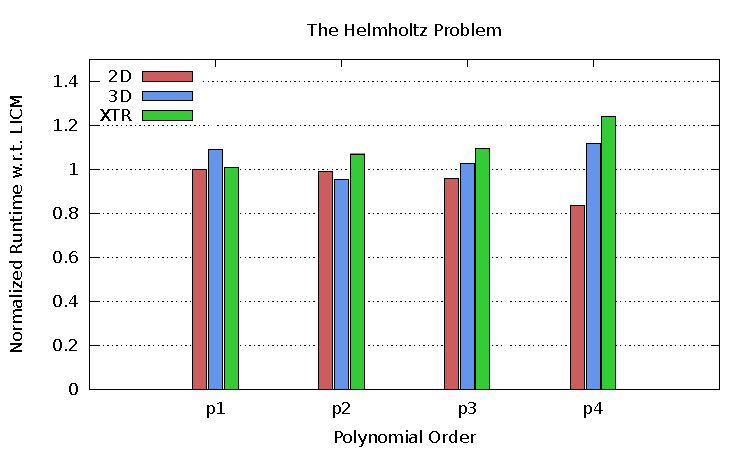
\includegraphics[scale=0.7]{Pictures/helmholtz-normalized.pdf}
\label{fig_first_case}}
\caption{Helmholtz}
\end{figure}

\begin{figure}[h]
\centerline{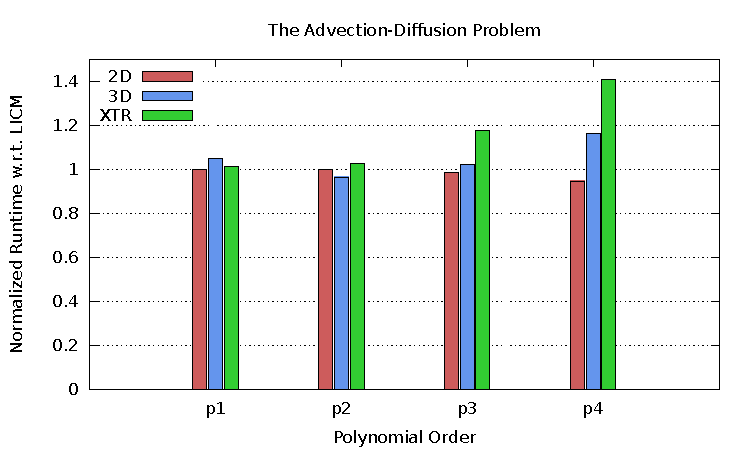
\includegraphics[scale=0.7]{Pictures/advdiff-normalized.pdf}
\label{fig_first_case}}
\caption{Advection-Diffusion}
\end{figure}

\begin{figure}[h]
\centerline{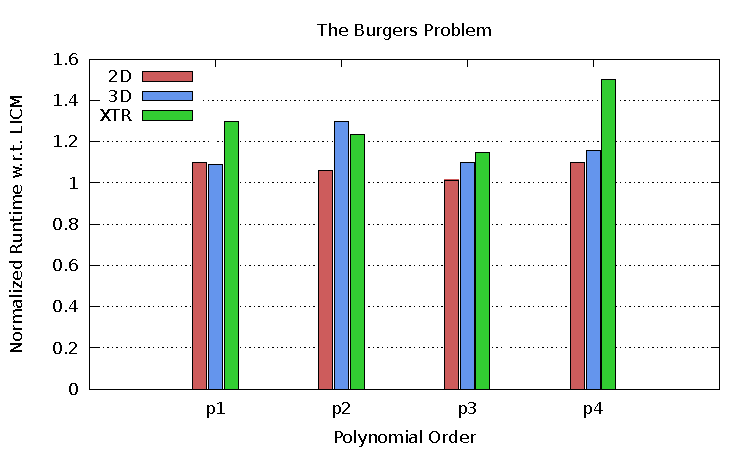
\includegraphics[scale=0.7]{Pictures/burgers-normalized.pdf}
\label{fig_first_case}}
\caption{Burgers}
\end{figure}

% We fix a specific loop permutation (i esterno perche minimizza.... swapping j or k, after LICM, is equivalent)

\section{Related Work}
%Show other work of people working on optimizations for computational science kernels. Inter-kernel vectorisation paper from Istvan. Previous work in FFC. Spencer et-al + Shin et. al. attempt to optimize computations that could benefit from using BLAS, but in practice they don't, due to the very small dgemm operations employed. Saday's model-driven SIMD code vectorisation for the tensor contraction engine.


\section{Conclusions}

%\subsubsection{Subsubsection Heading Here}
%Subsubsection text here.


% An example of a floating figure using the graphicx package.
% Note that \label must occur AFTER (or within) \caption.
% For figures, \caption should occur after the \includegraphics.
% Note that IEEEtran v1.7 and later has special internal code that
% is designed to preserve the operation of \label within \caption
% even when the captionsoff option is in effect. However, because
% of issues like this, it may be the safest practice to put all your
% \label just after \caption rather than within \caption{}.
%
% Reminder: the "draftcls" or "draftclsnofoot", not "draft", class
% option should be used if it is desired that the figures are to be
% displayed while in draft mode.
%
%\begin{figure}[!t]
%\centering
%\includegraphics[width=2.5in]{myfigure}
% where an .eps filename suffix will be assumed under latex, 
% and a .pdf suffix will be assumed for pdflatex; or what has been declared
% via \DeclareGraphicsExtensions.
%\caption{Simulation Results}
%\label{fig_sim}
%\end{figure}

% Note that IEEE typically puts floats only at the top, even when this
% results in a large percentage of a column being occupied by floats.


% An example of a double column floating figure using two subfigures.
% (The subfig.sty package must be loaded for this to work.)
% The subfigure \label commands are set within each subfloat command, the
% \label for the overall figure must come after \caption.
% \hfil must be used as a separator to get equal spacing.
% The subfigure.sty package works much the same way, except \subfigure is
% used instead of \subfloat.
%
%\begin{figure*}[!t]
%\centerline{\subfloat[Case I]\includegraphics[width=2.5in]{subfigcase1}%
%\label{fig_first_case}}
%\hfil
%\subfloat[Case II]{\includegraphics[width=2.5in]{subfigcase2}%
%\label{fig_second_case}}}
%\caption{Simulation results}
%\label{fig_sim}
%\end{figure*}
%
% Note that often IEEE papers with subfigures do not employ subfigure
% captions (using the optional argument to \subfloat), but instead will
% reference/describe all of them (a), (b), etc., within the main caption.


% An example of a floating table. Note that, for IEEE style tables, the 
% \caption command should come BEFORE the table. Table text will default to
% \footnotesize as IEEE normally uses this smaller font for tables.
% The \label must come after \caption as always.
%
%\begin{table}[!t]
%% increase table row spacing, adjust to taste
%\renewcommand{\arraystretch}{1.3}
% if using array.sty, it might be a good idea to tweak the value of
% \extrarowheight as needed to properly center the text within the cells
%\caption{An Example of a Table}
%\label{table_example}
%\centering
%% Some packages, such as MDW tools, offer better commands for making tables
%% than the plain LaTeX2e tabular which is used here.
%\begin{tabular}{|c||c|}
%\hline
%One & Two\\
%\hline
%Three & Four\\
%\hline
%\end{tabular}
%\end{table}


% Note that IEEE does not put floats in the very first column - or typically
% anywhere on the first page for that matter. Also, in-text middle ("here")
% positioning is not used. Most IEEE journals/conferences use top floats
% exclusively. Note that, LaTeX2e, unlike IEEE journals/conferences, places
% footnotes above bottom floats. This can be corrected via the \fnbelowfloat
% command of the stfloats package.




% conference papers do not normally have an appendix


% use section* for acknowledgement
\section*{Acknowledgment}


The authors would like to thank...





% trigger a \newpage just before the given reference
% number - used to balance the columns on the last page
% adjust value as needed - may need to be readjusted if
% the document is modified later
%\IEEEtriggeratref{8}
% The "triggered" command can be changed if desired:
%\IEEEtriggercmd{\enlargethispage{-5in}}

% references section

% can use a bibliography generated by BibTeX as a .bbl file
% BibTeX documentation can be easily obtained at:
% http://www.ctan.org/tex-archive/biblio/bibtex/contrib/doc/
% The IEEEtran BibTeX style support page is at:
% http://www.michaelshell.org/tex/ieeetran/bibtex/
%\bibliographystyle{IEEEtran}
% argument is your BibTeX string definitions and bibliography database(s)
%\bibliography{IEEEabrv,../bib/paper}
%
%% <OR> manually copy in the resultant .bbl file
%% set second argument of \begin to the number of references
%% (used to reserve space for the reference number labels box)
%\begin{thebibliography}{1}
%
%\bibitem{IEEEhowto:kopka}
%H.~Kopka and P.~W. Daly, \emph{A Guide to \LaTeX}, 3rd~ed.\hskip 1em plus
%  0.5em minus 0.4em\relax Harlow, England: Addison-Wesley, 1999.
%
%\end{thebibliography}
%

\bibliographystyle{plain}	% (uses file "plain.bst")
\bibliography{biblio}		% expects file "myrefs.bib"



% that's all folks
\end{document}


